%!TEX root = ../../Master.tex
\subsubsection{Block} % (fold)
\label{subsub:block}

Block er en klasse til håndtering af en klods. Klassen har ansvar for at holde styr på klodsens orientering samt placering i form af et koordinat for klodsens centrum. Dette opnås ved hjælp af klassens to funktioner, som er beskrevet herunder. \\

\textbf{img2base\_transform} \\
Denne funktion har til formål at transformere koordinatsættet fra billedet, som angives i pixels til koordinatsættet for robotten, som angives i cm.\\

Første del af funktionen står for at oversætte pixelkoordinater til koordinator i cm. Dette er gjort ved at finde antallet af pixels på en cm på billedet og derved dele alle pixel koordinator med dette. \\

Den sidste del består i at transformere billedkoordinatsættet til robotkoordinatsættet. De to koordinatsæt er illustret i \autoref{fig:img2base}, hvor koordinatsættet øverst i venstre side er for billedet og koordinatsættet nederst i midten er for robotten. Som figuren indikerer, kræver denne transformation både translation i x-aksens og y-aksens retning samt en rotation om både x- og z-aksen. \\

\fixme{Ændre 'Figure' til 'Figur'}

\begin{figure}[H]
\centering
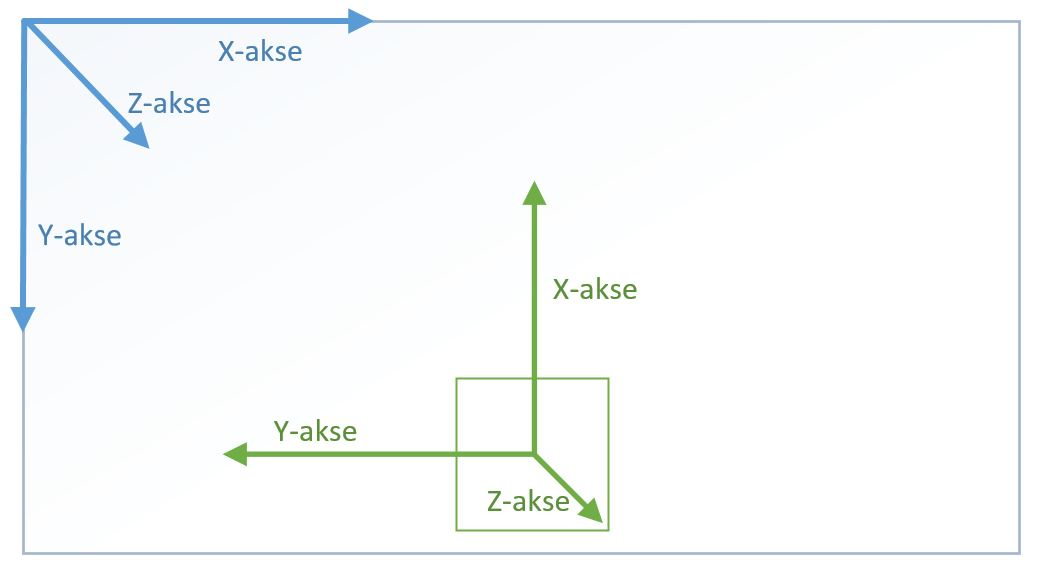
\includegraphics[scale=0.4]{images/img2base}
\caption{Billedkoordinatsæt og robotkoordinatsæt i forhold til bord.}
\label{fig:img2base}
\end{figure}

I implementeringen af dette oprettes derfor to matricer - en transformationsmatrix med både translation og rotation og en rotationsmatrix for den sidste rotation. Dette kan ses i \autoref{transformation}. Matrix A translaterer koordinaterne langs x- og y-aksen og roterer disse omkring x-aksen. Matrix B roterer koordinaterne om z-aksen. For at anvende disse matricer, skal koordinattet, som skal transformeres, være et homogent koordinat.

\begin{lstlisting}[caption=Matricer til transformation., label=transformation, language=Python]
A = np.matrix([
    [1, 0,           0,            tx],
    [0, cos(thetax), -sin(thetax), ty],
    [0, sin(thetax), cos(thetax),  tz],
    [0, 0,           0,            1 ]
    ])

B = np.matrix([
    [cos(thetaz),  sin(thetaz), 0, 0],
    [-sin(thetaz), cos(thetaz), 0, 0],
    [0,            0,           1, 0],
    [0,            0,           0, 1]
    ])
\end{lstlisting}


\textbf{img2joint1\_transform} \\
Denne funktion er en hjælpefunktion, som bruges til at rotere en vektor $[x,y]$ omkring z-aksen. Dette gøres som ved matrix B i \autoref{transformation}. \\


\textbf{find\_orientation} \\
Denne funktion har til formål at bestemme orienteringen på klodsen i forhold til robotten. Klodsen har to orienteringer, da den har to ikke parallelle sider. \\

Fra den tidligere billedprocessering kendes klodsens fire hjørner. Ud fra disse fire hjørner fås to vektorer, som har samme orientering som klodsens to sider. Vinklen mellem hver af disse to vektorer og x-aksen er orienteringen. Vektoren findes ved at trække de to punkter fra hinanden og viklen opnås ved at bruge tangens på $y/x$. Implementationen af dette ses i \autoref{orientation}. \\

Den sidste detalje er så, at orienteringen ikke skal rejnes ud fra basens x-akse, men i stedet ud fra den x-akse, som følger robottens første rotationsled. Derfor transformeres vektorens koordinater til dette koordinatsystem, som er roteret lige så meget om z-aksen, som robottens første rotationsled, $q1$. Derved kan den beregnede orientation bruges som input til robottens fjerde rotationsled, hvor gripperen er monteret på. \\

\begin{lstlisting}[caption=Funktion til at finde orientering på en klods., label=orientation, language=Python]
def find_orientation(self, q1):
    min_theta = 0

    for i in range(0, 2):
        corner1 = self.img2joint1_transform(self.corners[i][0], self.corners[i][1], q1)
        corner2 = self.img2joint1_transform(self.corners[i+1][0], self.corners[i+1][1], q1)

        dx = corner2[0] - corner1[0]
        dy = corner2[1] - corner1[1]

        theta = atan2(dy, dx)

        if abs(theta) < abs(min_theta) or i == 0:
            min_theta = theta

    return min_theta
\end{lstlisting}
% subsubsection block (end)